\documentclass{beamer}
\usetheme{default}

\setbeamertemplate{itemize items}[ball]
\setbeamertemplate{itemize subitem}{-}
\setbeamertemplate{itemize subsubitem}{>}

%\usefonttheme{professionalfonts} % using non standard fonts for beamer
%\usepackage{fontspec}
%\setsansfont{Graphik}

\title{Model Documentations\\Airport Arrivals in a Post-Pandemic World}
\author{Vincent Leonardo\\Sarah Wong I-Mae\\Sarah Ramjoo}
\begin{document}
\begin{frame}[plain]
    \maketitle
\end{frame}
\begin{frame}{Overview}
	\tableofcontents
\end{frame}
\section{Dependencies}
\begin{frame}{Dependencies}
	\begin{itemize}
		\item Internet connection for the different libraries imported by the model.
		\item A modern browser updated within this year (2021) is preferred due to some newer CSS dependencies. This model is also compatible with mobile browsers.
		\item This model can also be accessed at \url{https://github.vinleonardo.com/sma-airport-model/}.
		\item The webpage version of this documentation can be accessed at \url{https://github.vinleonardo.com/sma-airport-model/documentations}
	\end{itemize}
\end{frame}

\section{User manual}
\subsection{Objectives of the model}
\begin{frame}{Objectives of the model}
	\begin{itemize}
		\item The objective of this simulation is to bring a passenger from the the plane (left border) and out of the system.
		\item There are two ways of exiting: one is through the normal way of clearing the defined stations, the other is when, if there is a testing station, the passenger tested positive for COVID-19.
		\item  The behaviour of the passengers is that they will all walk at the same speed without social distancing, always moving forward, and selection of queues will be done either randomly or in choosing the shortest queue (user-set probability). Moreover, for COVID-19 testings, everything is assumed to be 100\% accurate.
	\end{itemize}
\end{frame}
\subsubsection{Immigration station}
\begin{frame}{Immigration station}
	\begin{figure}
		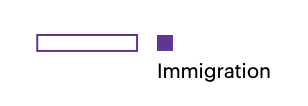
\includegraphics[scale=1]{../img/immigration}
		\caption{Immigration station}
		
	\end{figure}
	\begin{itemize}
		\item The immigration station is comprised of pair-wise queue lanes and booths.
		\item The behaviour is a simple one in that passengers will queue and wait for their turn to go next into the booth.
	\end{itemize}
\end{frame}

\subsubsection{Testing station}
\begin{frame}{Testing station}
	\begin{figure}
		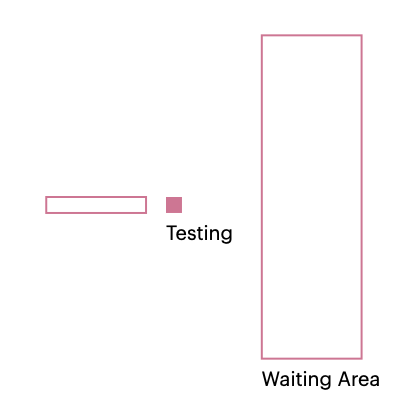
\includegraphics[scale=0.6]{../img/testing}
		\caption{Testing station}
		
	\end{figure}
	\begin{itemize}
		\item The testing station is similar to the immigration station.
		\item But, after the booth, the passengers go into a waiting area where they randomly choose their sitting positions to wait for a set amount of time.
	\end{itemize}
\end{frame}

\subsubsection{Baggage station}
\begin{frame}{Baggage station}
	\begin{figure}
		
		\begin{columns}
			\column{0.4\textwidth}
			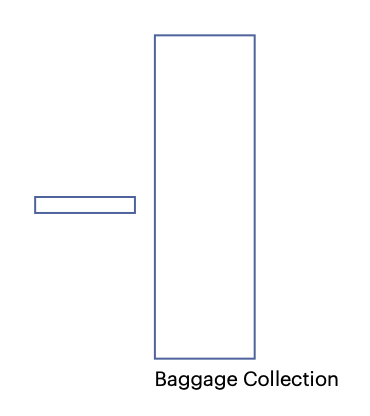
\includegraphics[scale=0.6]{../img/baggage}
			\caption{Baggage station}
			\column{0.6\textwidth}
			\begin{itemize}
				\item The baggage area is simple. It contains a lane to enter in (which is not a queue) and a baggage area afterwards. 
				\item This is, of course, assuming that the baggages are not on carousels as per normal, but left down on the ground due to the special circumstances. 
				\item The passenger will try to look for their baggages within this area and then leave.
			\end{itemize}
		\end{columns}
	\end{figure}
\end{frame}

\subsection{UI elements}
\begin{frame}{UI elements - before simulation box}
	The lines before the simulation box denote the changing variables during the simulation. This includes the time within the current simulation, the number of exited passengers within the current simulation, and the average time taken per passenger within the current simulation along with the average time taken to finish one simulation and its standard deviation over the set amount of simulations.
	\begin{figure}
		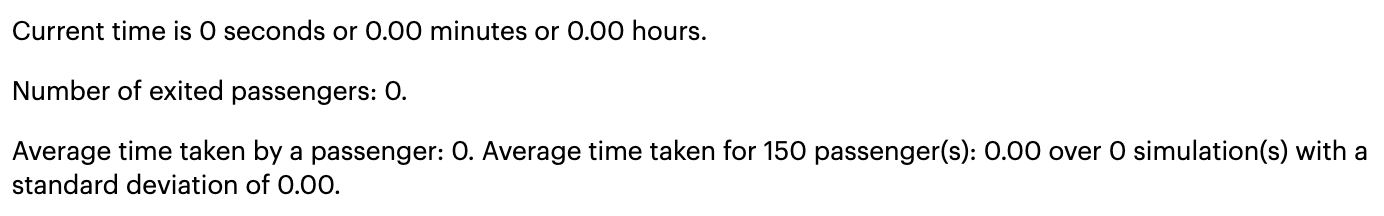
\includegraphics[width=\linewidth]{../img/befSimBox}
		\caption{What is seen before the simulation box}
	\end{figure}

	Before setting any stations, the simulation box will be an empty box with a black border.
	
\end{frame}

\begin{frame}{UI elements - after simulation box}
	Below the simulation box, there are two graphs: one to track the average time taken per passenger within one simulation run, and the other one to track the average time taken to finish one simulation run.
	\begin{figure}
		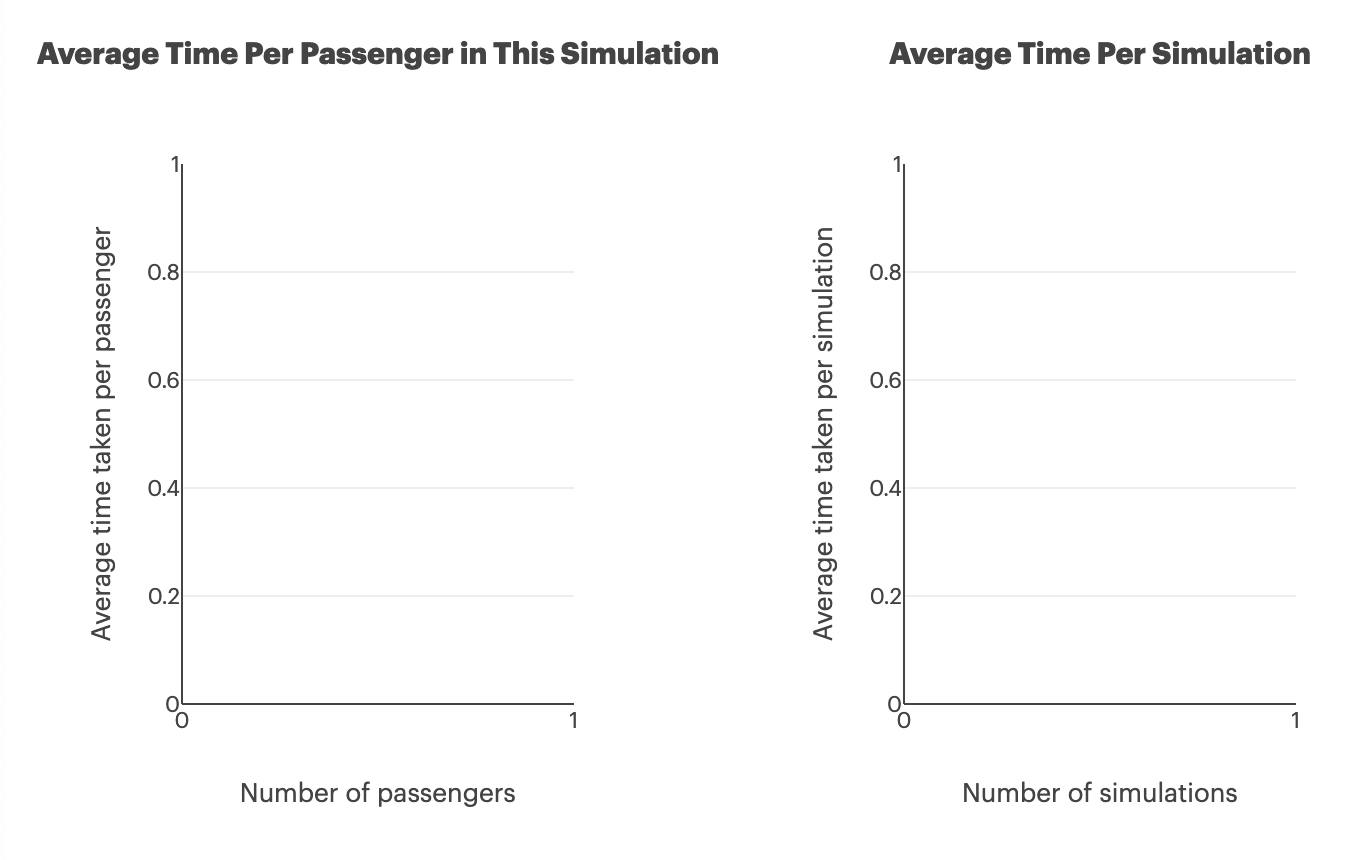
\includegraphics[scale=0.3]{../img/graphs}
		\caption{What is seen after the simulation box}
	\end{figure}
	
\end{frame}

\begin{frame}{UI elements - after simulation box}
	Right below that, there are control buttons to start, pause, and reset the simulations. It is also possible to download the data collected for the time taken per simulation over one or multiple simulations as a CSV file.
	\begin{figure}
		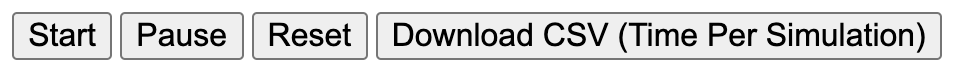
\includegraphics[scale=0.3]{../img/buttons}
		\caption{What is seen after the simulation box}
	\end{figure}
	
\end{frame}

\subsection{Inputs}

\begin{frame}{Inputs}
	There are three different sections covering different aspects of the simulation. 
	\begin{itemize}
		\item One is Stations, which covers both the layout of the stations within the simulation box and the global simulation settings. 
		\item The next one is Station Parameters, which is used to customise how many booths or lanes each station has. 
		\item The final one is Agent Parameters, which control the agents' behaviours and time taken to go through each station.
	\end{itemize}
	
	\begin{figure}
		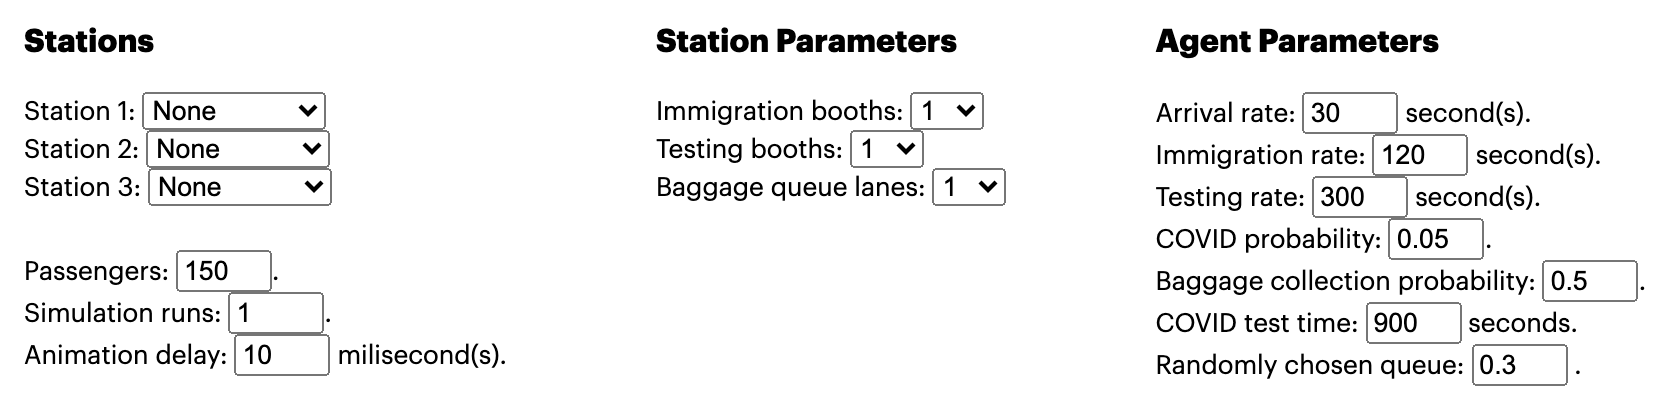
\includegraphics[scale=0.3]{../img/inputs}
		\caption{Inputs}
	\end{figure}
	
\end{frame}

\subsubsection*{Stations}

\begin{frame}{Inputs - Stations}
	There must be at least one choice of station for the simulation to run. The station numbers correspond to their position on the simulation box from left to right. For example, the picture below shows when Station 1 is Immigration, Station 2 is Testing, and Station 3 is Baggage.
	
	\begin{figure}
		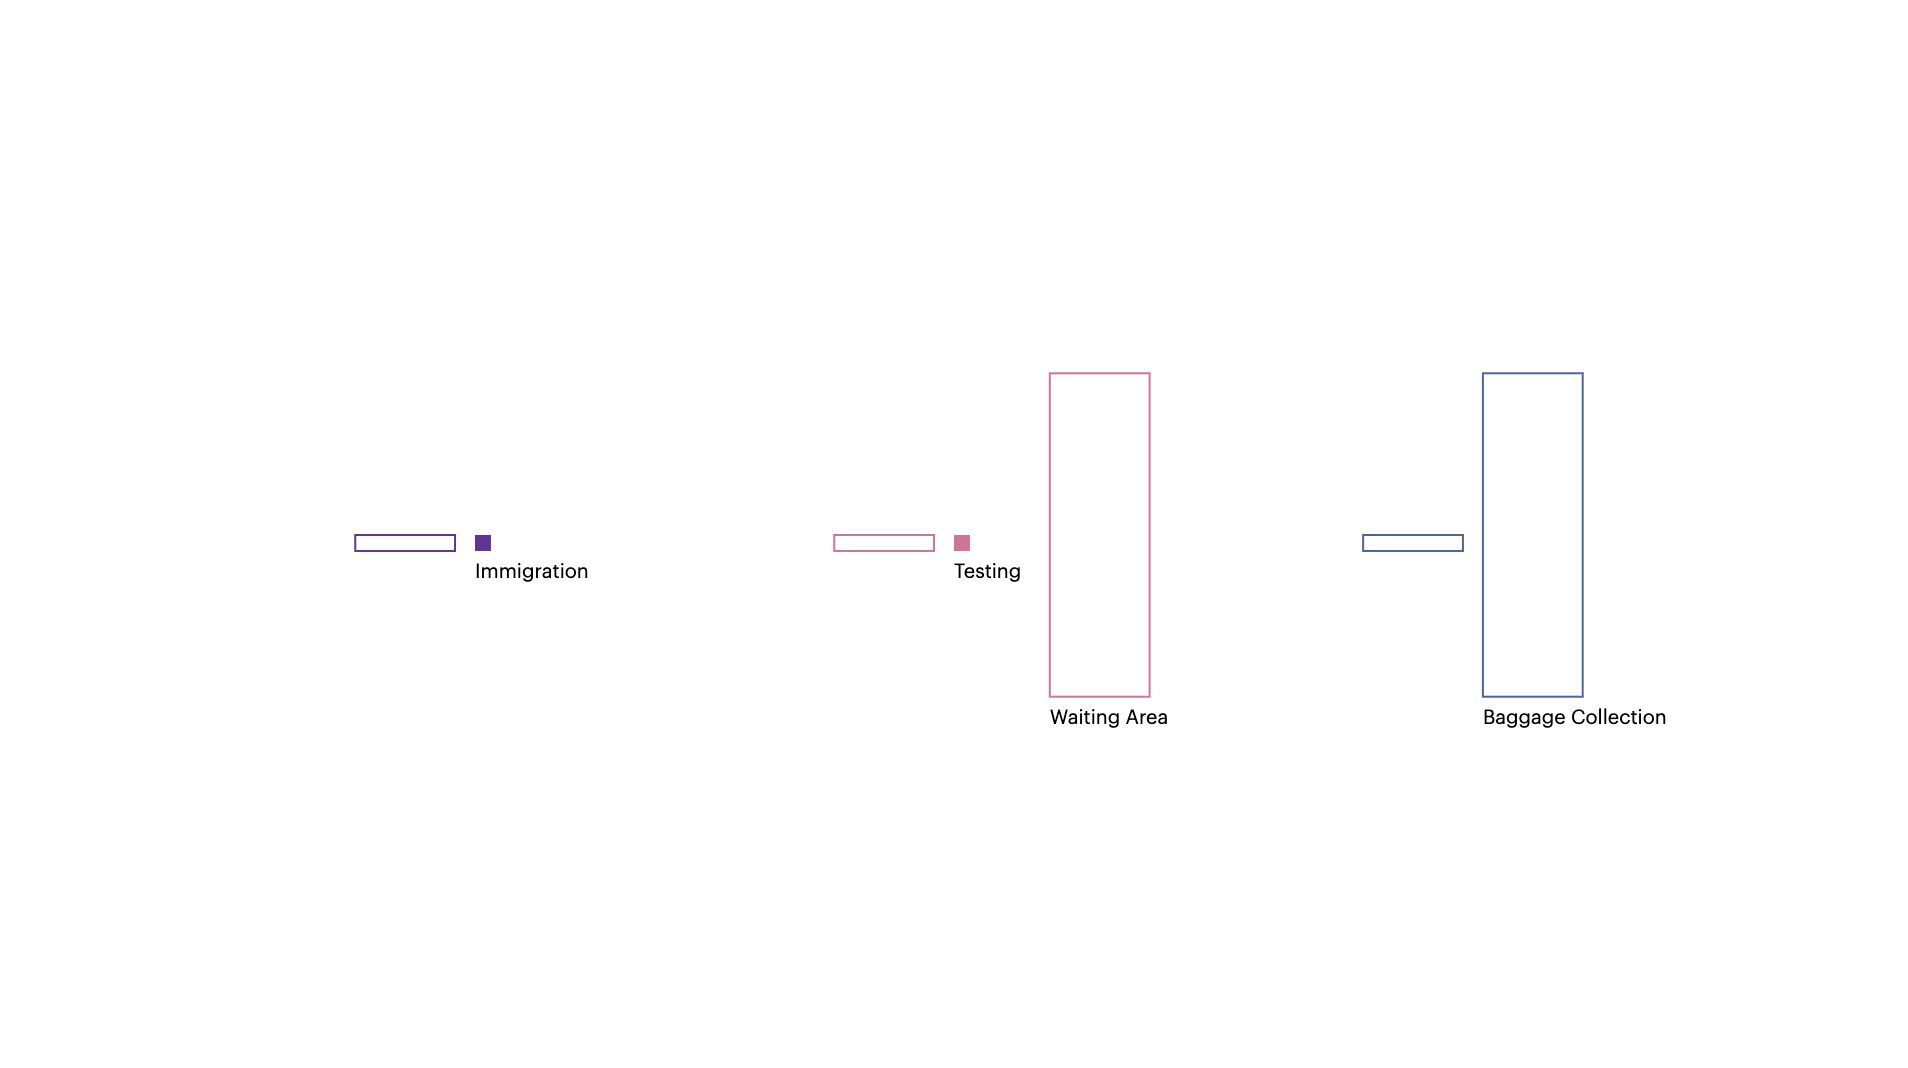
\includegraphics[scale=0.2]{../img/example1}
		\caption{Example of model set}
	\end{figure}
	
\end{frame}

\subsubsection*{Station Parameters}
\begin{frame}{Inputs - Station Parameters}
	\begin{figure}
		
		\begin{columns}
			\column{0.4\textwidth}
			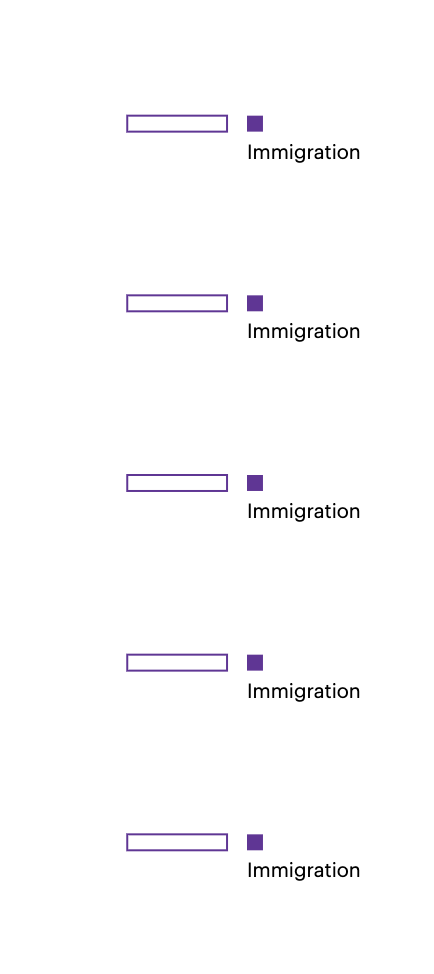
\includegraphics[scale=0.4]{../img/example2}
			\caption{Multiple immigration booths}
			\column{0.6\textwidth}
			The dropdowns denote the amount (from one to ten) of booths, queues, or lanes provided in the simulation for each station. An example for when the immigration booth is set to have five booths is as follows.
		\end{columns}
	\end{figure}
\end{frame}

\subsubsection*{Agent Parameters}

\begin{frame}{Inputs - Agent Parameters}
	The rates that are denoted in seconds will be converted into their per-second probability (its inverse), excepting the COVID test time, which is a definite time delay. This meant that the probability, for example, of an arrival rate of 30 seconds will be 1/30 per second.
	
	\begin{itemize}
		\item Arrival rate: the mean time taken for each passenger to enter the simulation.
		\item Immigration rate: the mean time to clear immigration for each passenger
		\item Testing rate: the mean time to clear the testing booth.
		\item COVID probability: the probability of each passenger having COVID.
		\item Baggage collection probability: the probability that when a passenger reaches the baggage area, their baggage is found.
		\item COVID test time: the time taken to clear the COVID test.
		\item Randomly chosen queue: the probability that a passenger will deviate from the rational queue choice (shortest queue).
	\end{itemize}
\end{frame}
\section{Behaviours and code}

\begin{frame}{Behaviours and code}
	This is going to be a high level description of the model, written in the perception of an individual agent. The animations are done using the D3.js library.
	\begin{figure}
		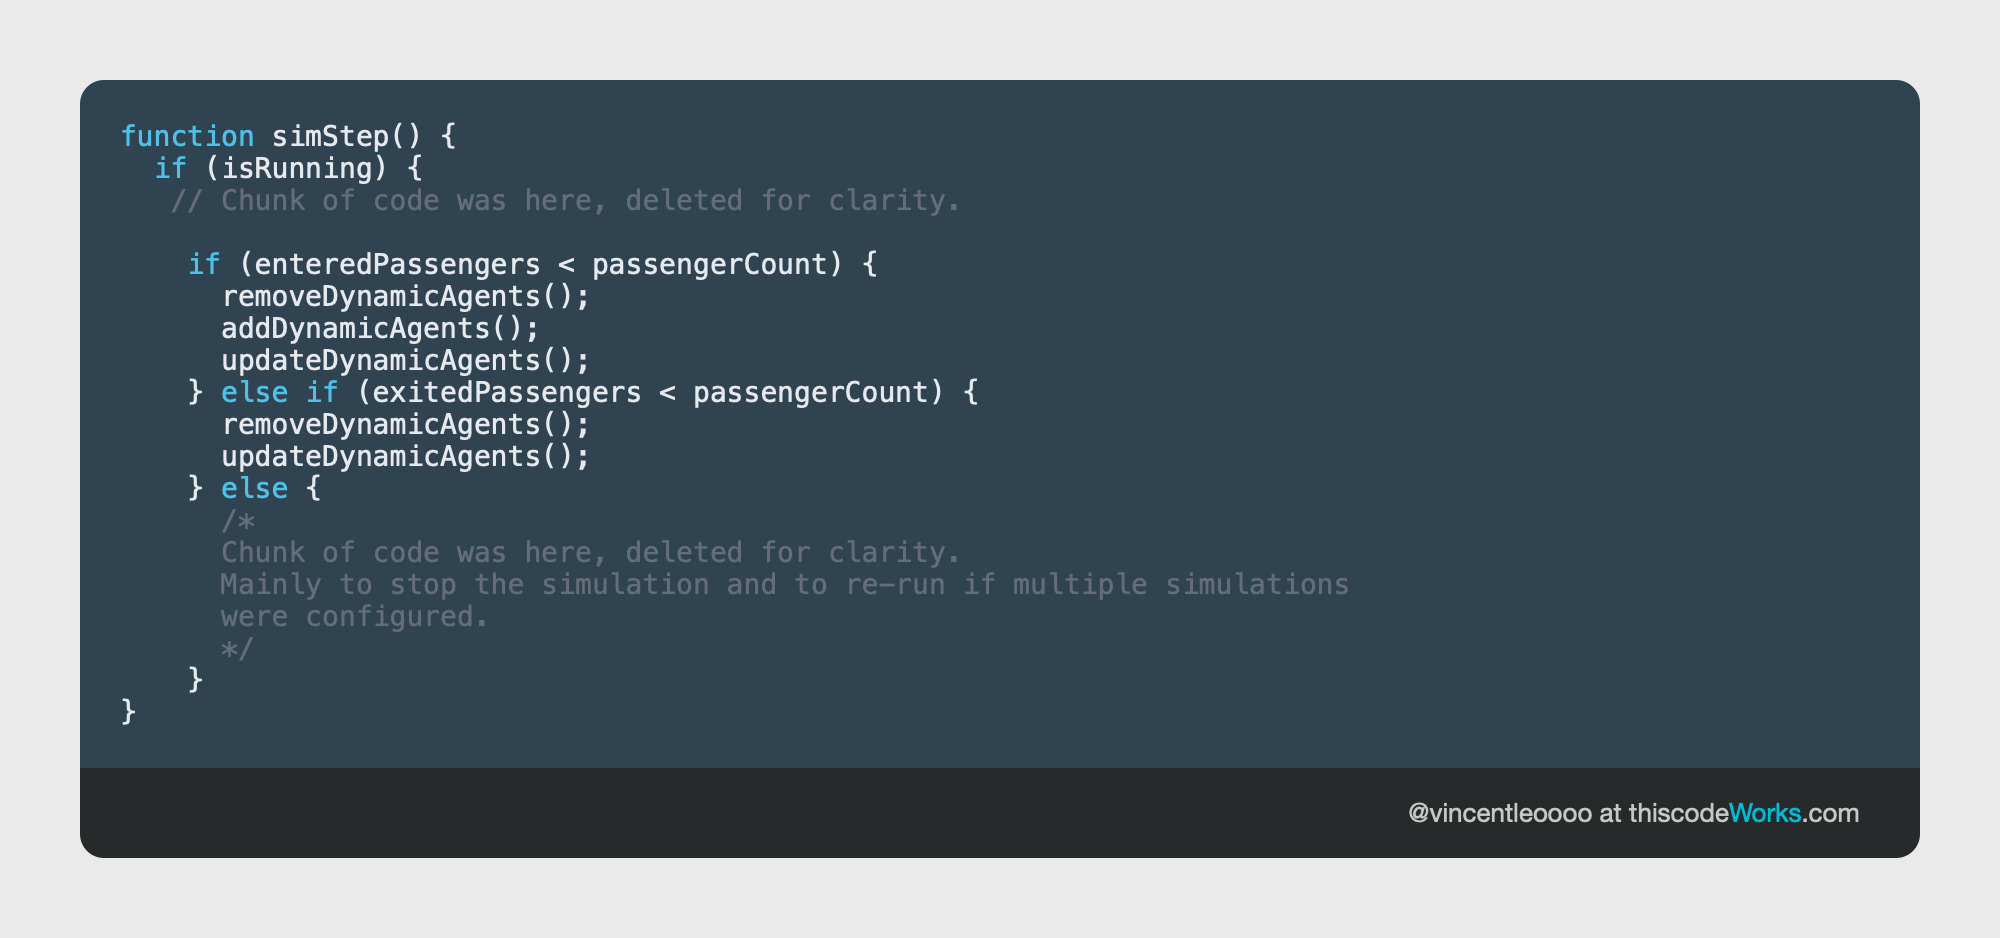
\includegraphics[width=\linewidth]{../img/high-level-process}\caption{High level overview}
	\end{figure}
\end{frame}

\begin{frame}{Behaviours and code}
	
	The code shown in the last slide shows the process for each second passing. Firstly, it is the garbage collection. This means that it will try to clear out whichever agent is at the going out state. Afterwards, it will create new passengers based on the rates set by the user as long as the number of passengers does not exceed the specified amount of passengers. It will then update the positions of all the agents in the simulation based on their target locations.
\end{frame}

\subsection{Removing passengers}

\begin{frame}{Removing passengers}
	
	In removing the passengers, it deletes both the passengers data and the data associated with the animation.
	
	\begin{figure}
		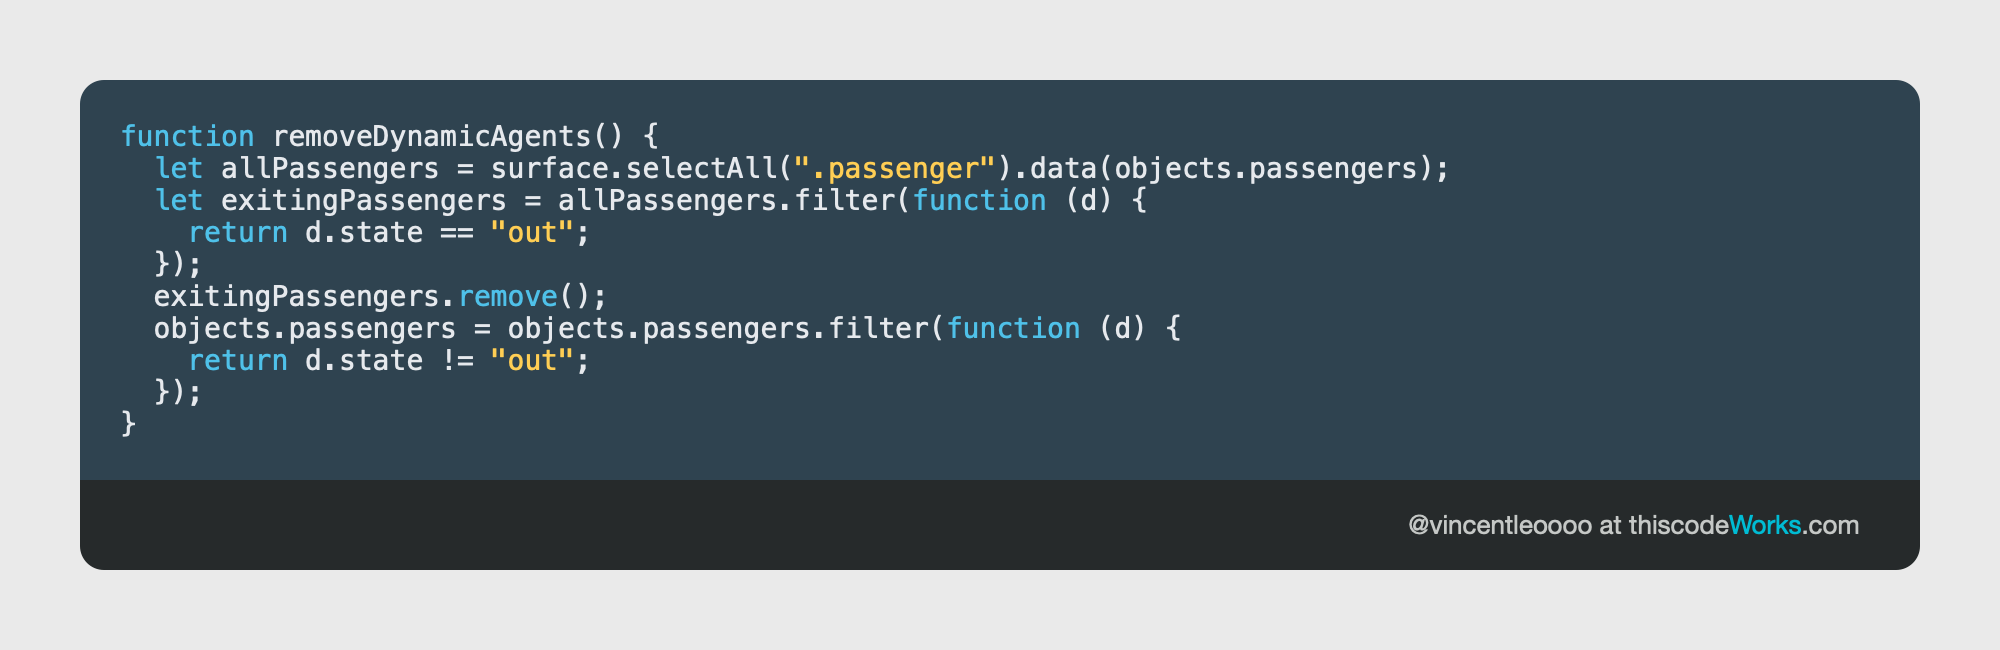
\includegraphics[width=\linewidth]{../img/remove-passengers}\caption{Removing passengers}
	\end{figure}
\end{frame}

\subsection{Adding passengers}

\begin{frame}{Adding passengers}
	
	\begin{itemize}
		\item In this case, it will follow a process of finding the next station.
		\item It will either choose the queue lane for the next station rationally based on queue lengths or based on random choice. This parameter is set by the user. 
		\item Afterwards, other attributes are assigned to keep track of its state. The user's choice for COVID infected probability will affect how many passengers have COVID.
		\item Code snippet can be seen at \url{https://www.thiscodeworks.com/61b4b094fe9bbd0015d5e7f3} since it is too long to be seen here.
	\end{itemize}
	
	
\end{frame}

\subsection{Updating passengers}
\begin{frame}{Updating passengers}
	
	\begin{itemize}
		\item In updating the passenger, there will be roughly two different states. One is when the passenger is still on the way to a target, and one where the passenger has reached a target. Depending on the station, the passenger will do different things.
		\item Code snippet can be seen at \url{https://www.thiscodeworks.com/61b4b185fe9bbd0015d5e7f4} since it is too long to be seen here.
		
	\end{itemize}
	
	
\end{frame}
\begin{frame}{Updating passengers}
	
	\begin{itemize}
		\item At the immigration booth, the passenger will queue up until it is their turn. After coming out of the booth, it will select the next station. At the testing booth, the passenger will also queue up to get tested. Afterwards, it is a free seating environment within the area used to wait for test results. At the baggage collection area, the passenger will go through the lanes into a space where the baggages are placed. They will then try to find their baggages. This probability is set by the user. If the next station is to go out, they will then proceed to go to the exit node.
		\item For COVID patients who are screened during testing, they will go out via a different path, thus reducing their time taken to go through the simulation.
		
	\end{itemize}
	
	
\end{frame}

\subsection{Area creation and modularity}
\begin{frame}{Area creation and modularity}
	\begin{itemize}
		\item JavaScript objects
		\item Area creation
		\item Tracking states and substates
	\end{itemize}
\end{frame}

\subsubsection*{JavaScript objects}
\begin{frame}{JavaScript objects}
	The example in the next slide shows the different ways to get keys or values within an object. This is how the model was able to find the positions of the stations based on what is set by the user and to connect the pieces together such that the passenger can find the next station and hence the queue. The object keys associated with queues are always called \texttt{\{station\} + Queue}. This leads to the stations behaving like Lego blocks, being able to connect with any other station with a standard input/output.
\end{frame}

\begin{frame}{JavaScript objects}
	\begin{figure}
		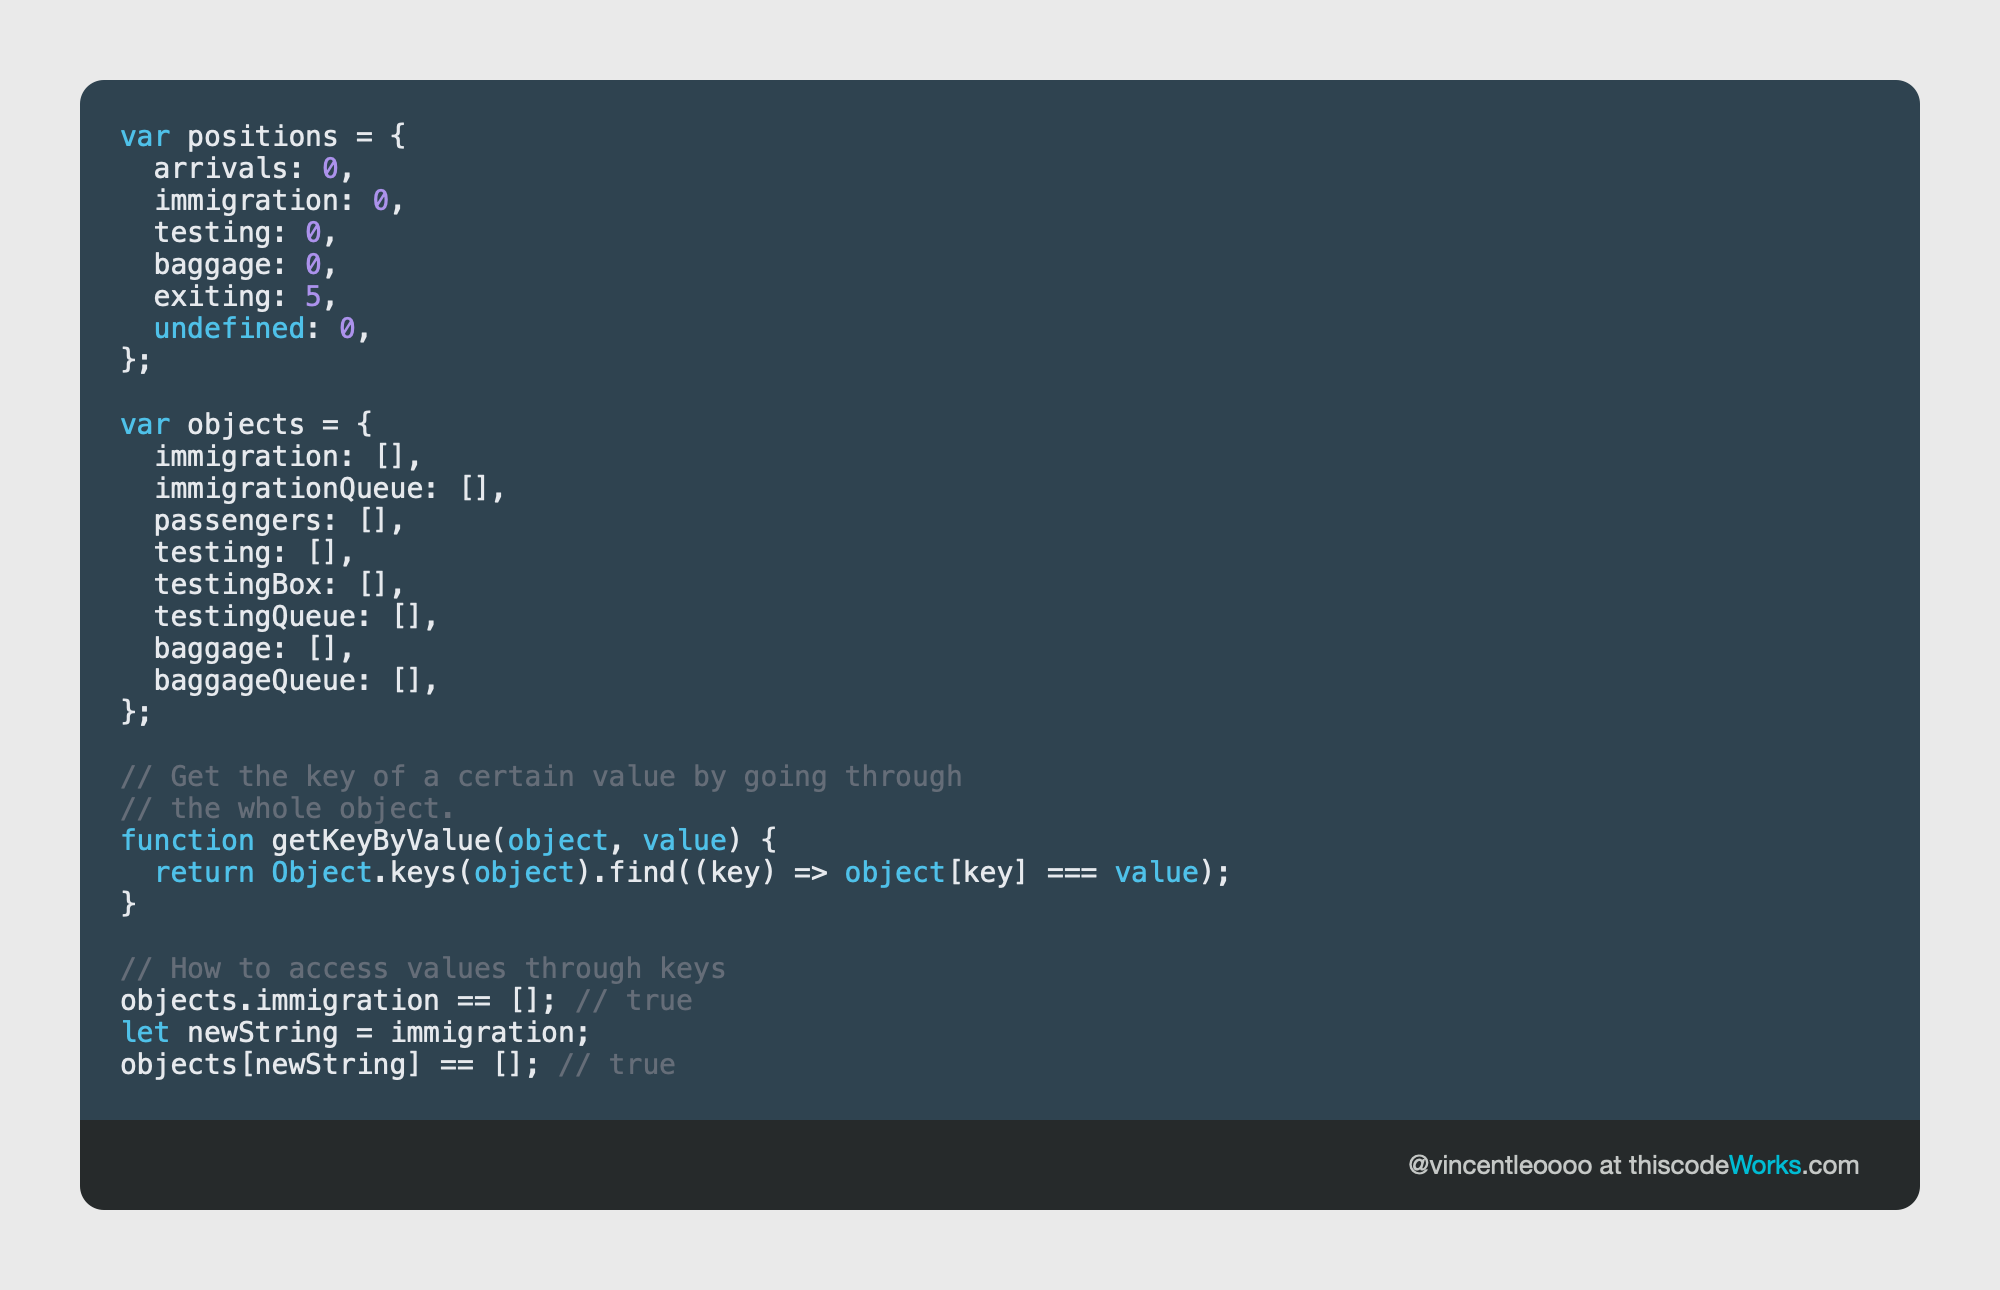
\includegraphics[width=\linewidth]{../img/objects-and-extraction-of-key-value-pairs}\caption{JavaScript hacks}
	\end{figure}
\end{frame}

\subsubsection*{Area creation}
\begin{frame}{Area creation}
	The creation of the areas will depend on whether the positions of the stations are defined (>0 in this case). Depending on the number of queues or booths set, the \texttt{objects} object will be modified where the stations' booths or queues will be added in such that it can be generated later on. On the next slide is an example for the immigration booth.
\end{frame}

\begin{frame}{Area creation}
	\begin{figure}
		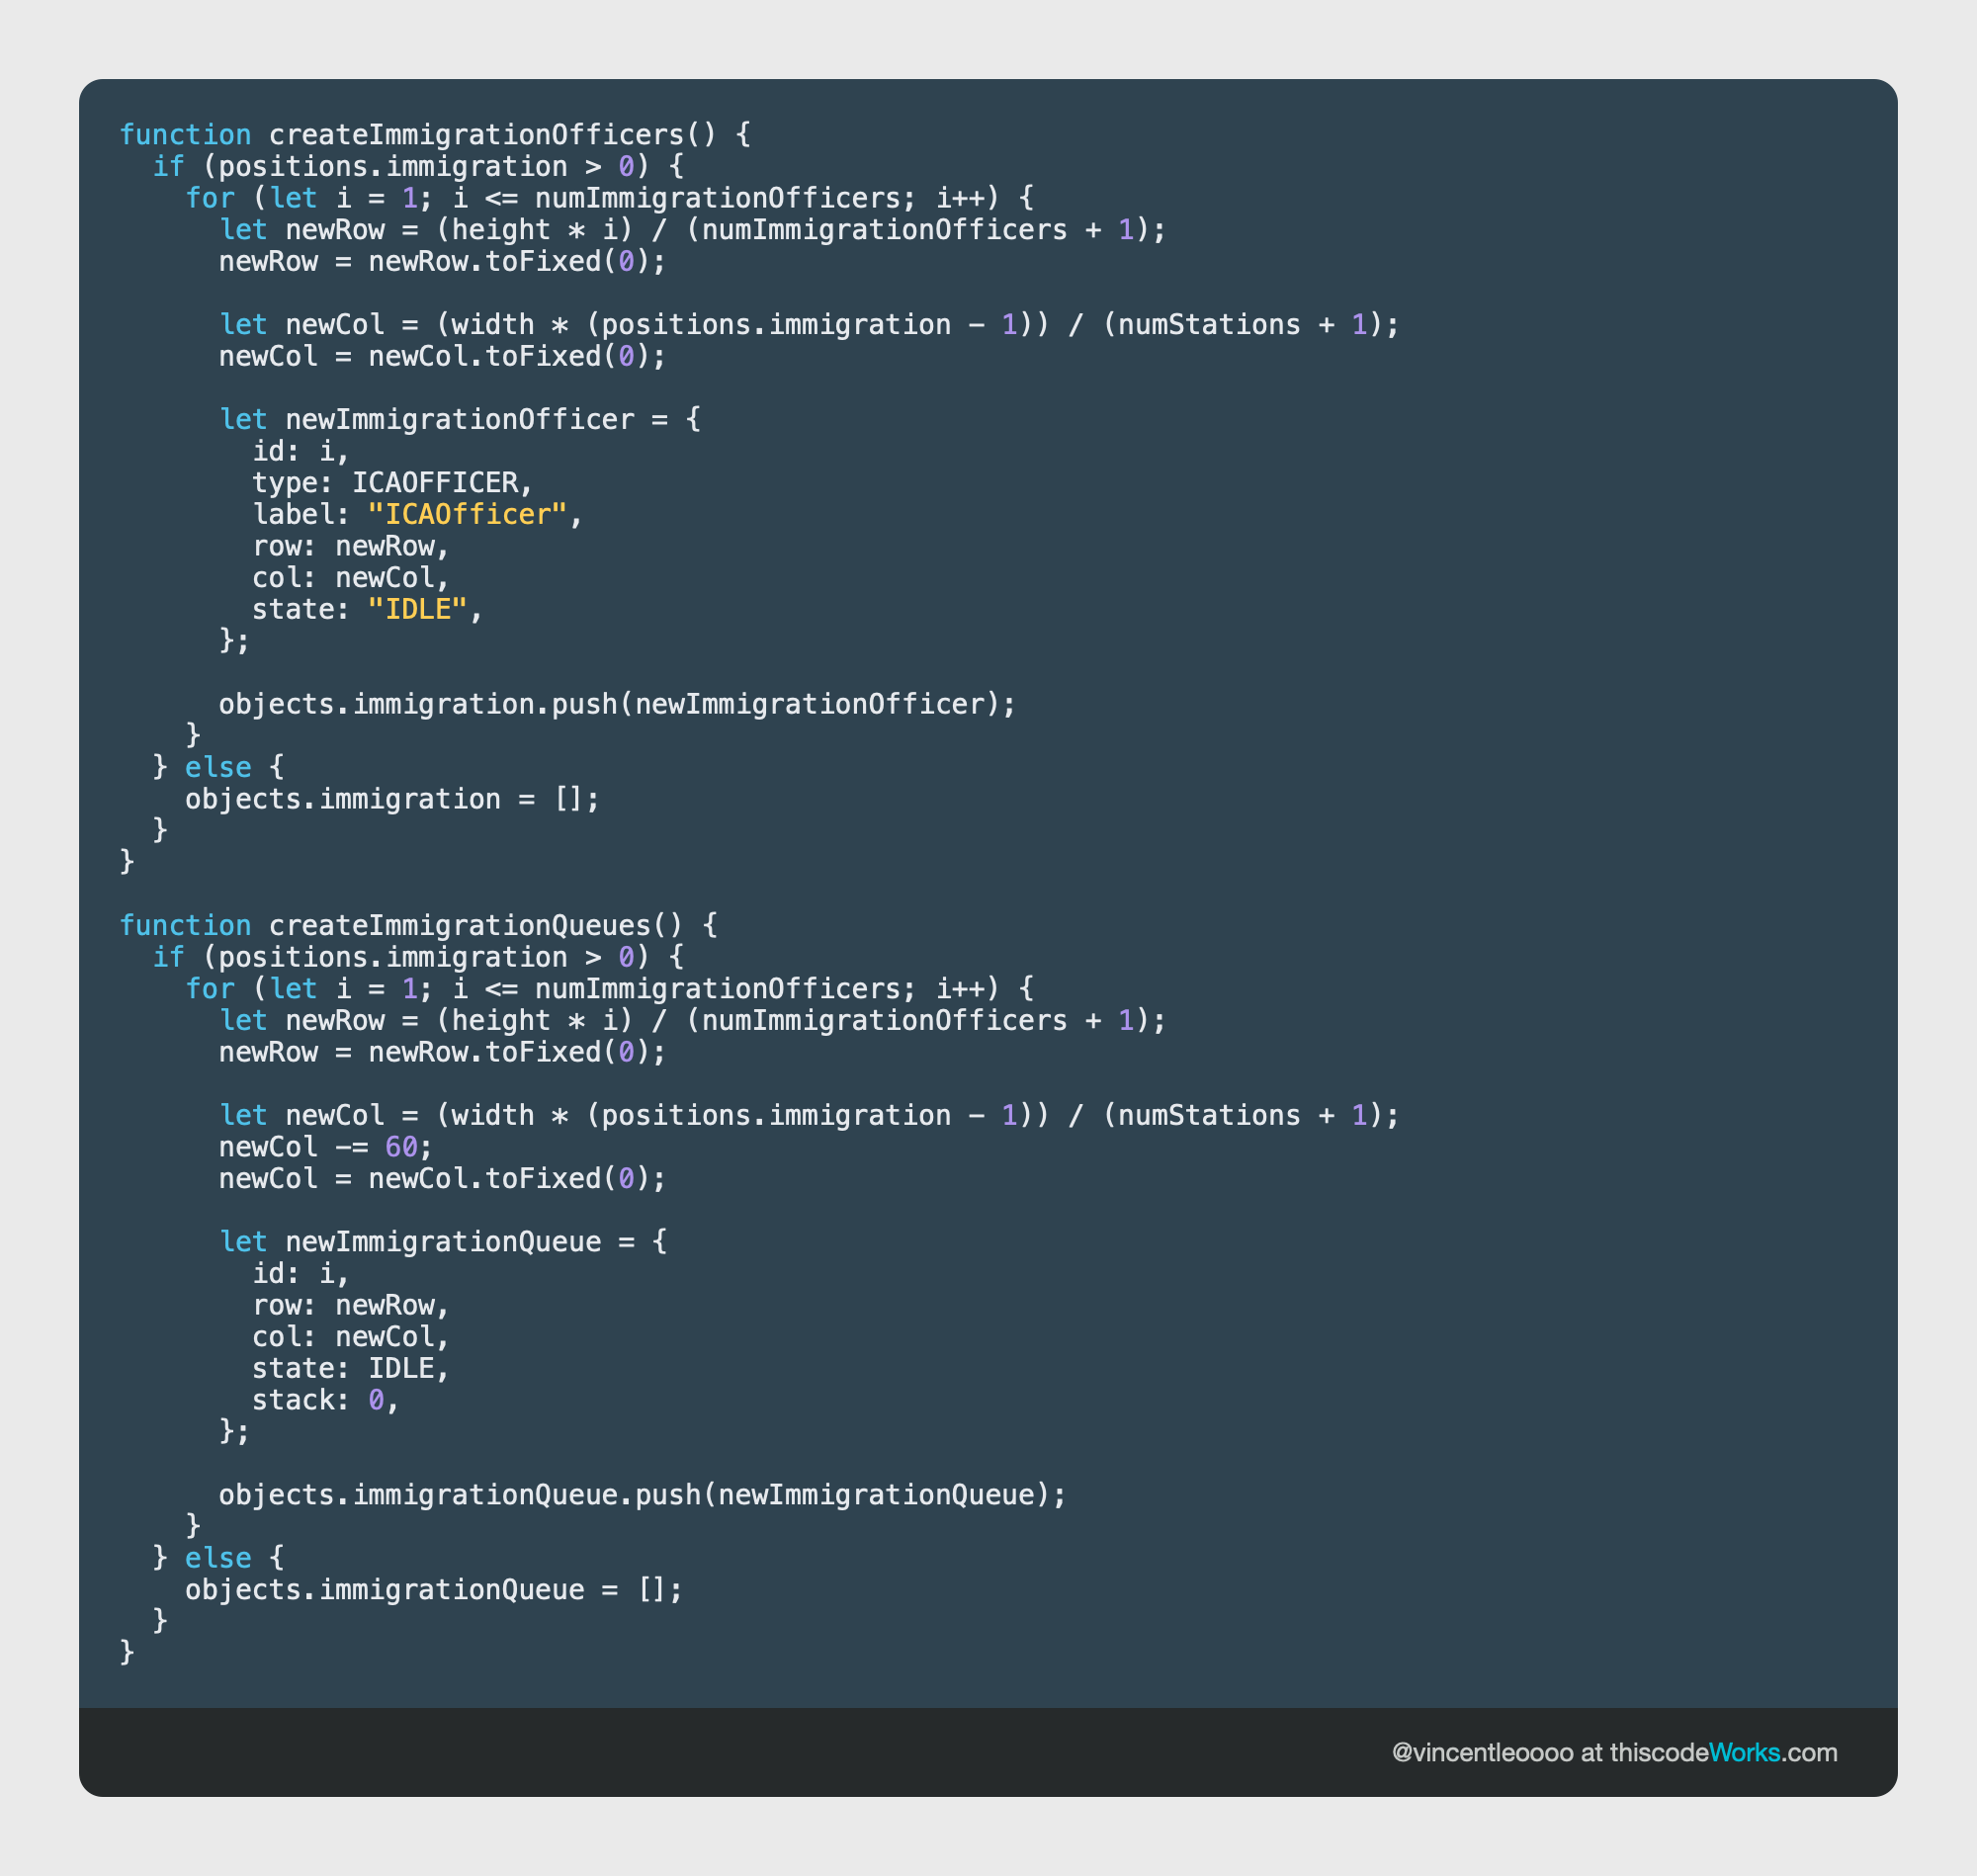
\includegraphics[scale=0.1]{../img/create-a-station-and-its-queues}\caption{Area creation}
	\end{figure}
\end{frame}

\subsubsection*{Tracking states and substates}
\begin{frame}{Tracking states and substates}
	The passengers have a \texttt{state} to denote which station to go, and a \texttt{queueState} to denote which part of each station to go to. They also have the \texttt{station} integer key to denote which part of the simulation box they are in, and as such they can track their progress and go find which station is in the next part using the tricks mentioned above.
\end{frame}

\subsection{Front-end niceties}
\begin{frame}{Front-end niceties}
	\begin{itemize}
		\item Inputs and value-safety
		\item Plots
		\item Downloads
	\end{itemize}
\end{frame}

\subsubsection*{Inputs and value-safety}
\begin{frame}{Inputs and value-safety}
	These are some of the functions that help to key in inputs from the front-end and to ensure that they are tenable.
	\begin{figure}
		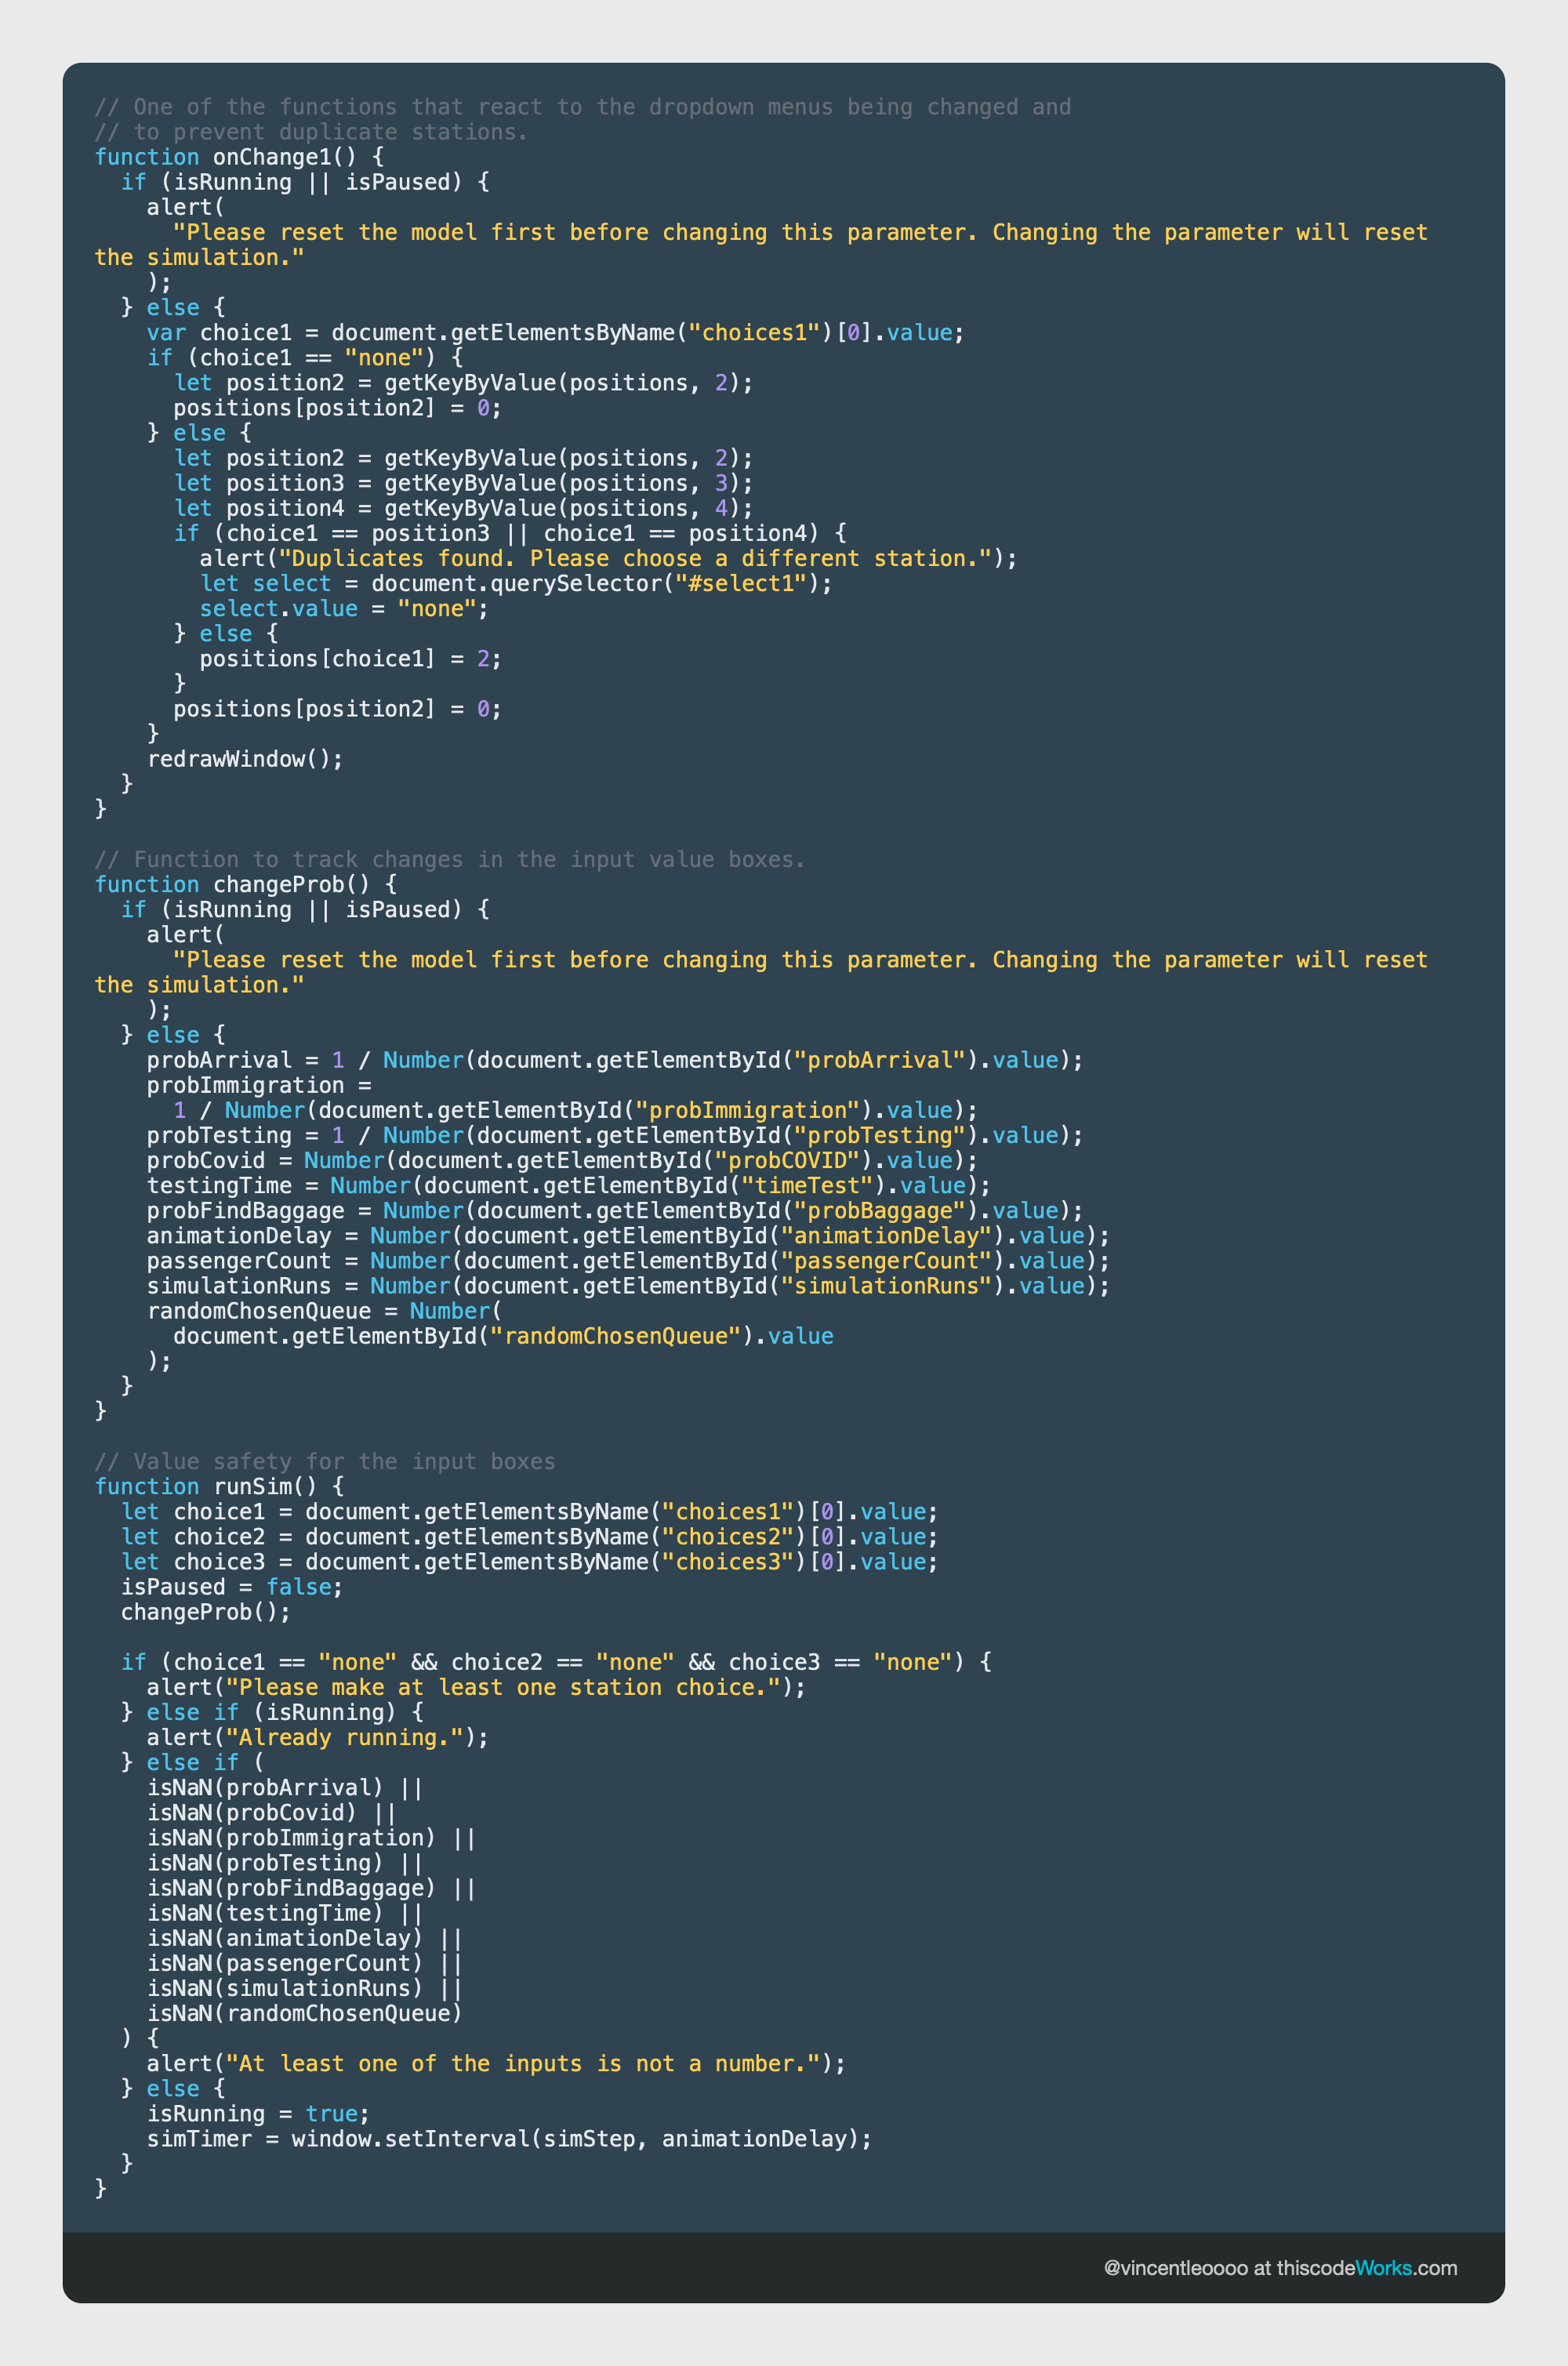
\includegraphics[scale=0.06]{../img/changing-things-on-the-front-end}\caption{Front-end inputs framework}
	\end{figure}
\end{frame}

\subsubsection*{Plots}
\begin{frame}{Plots}
	The plots are made using Plotly.
	\begin{figure}
		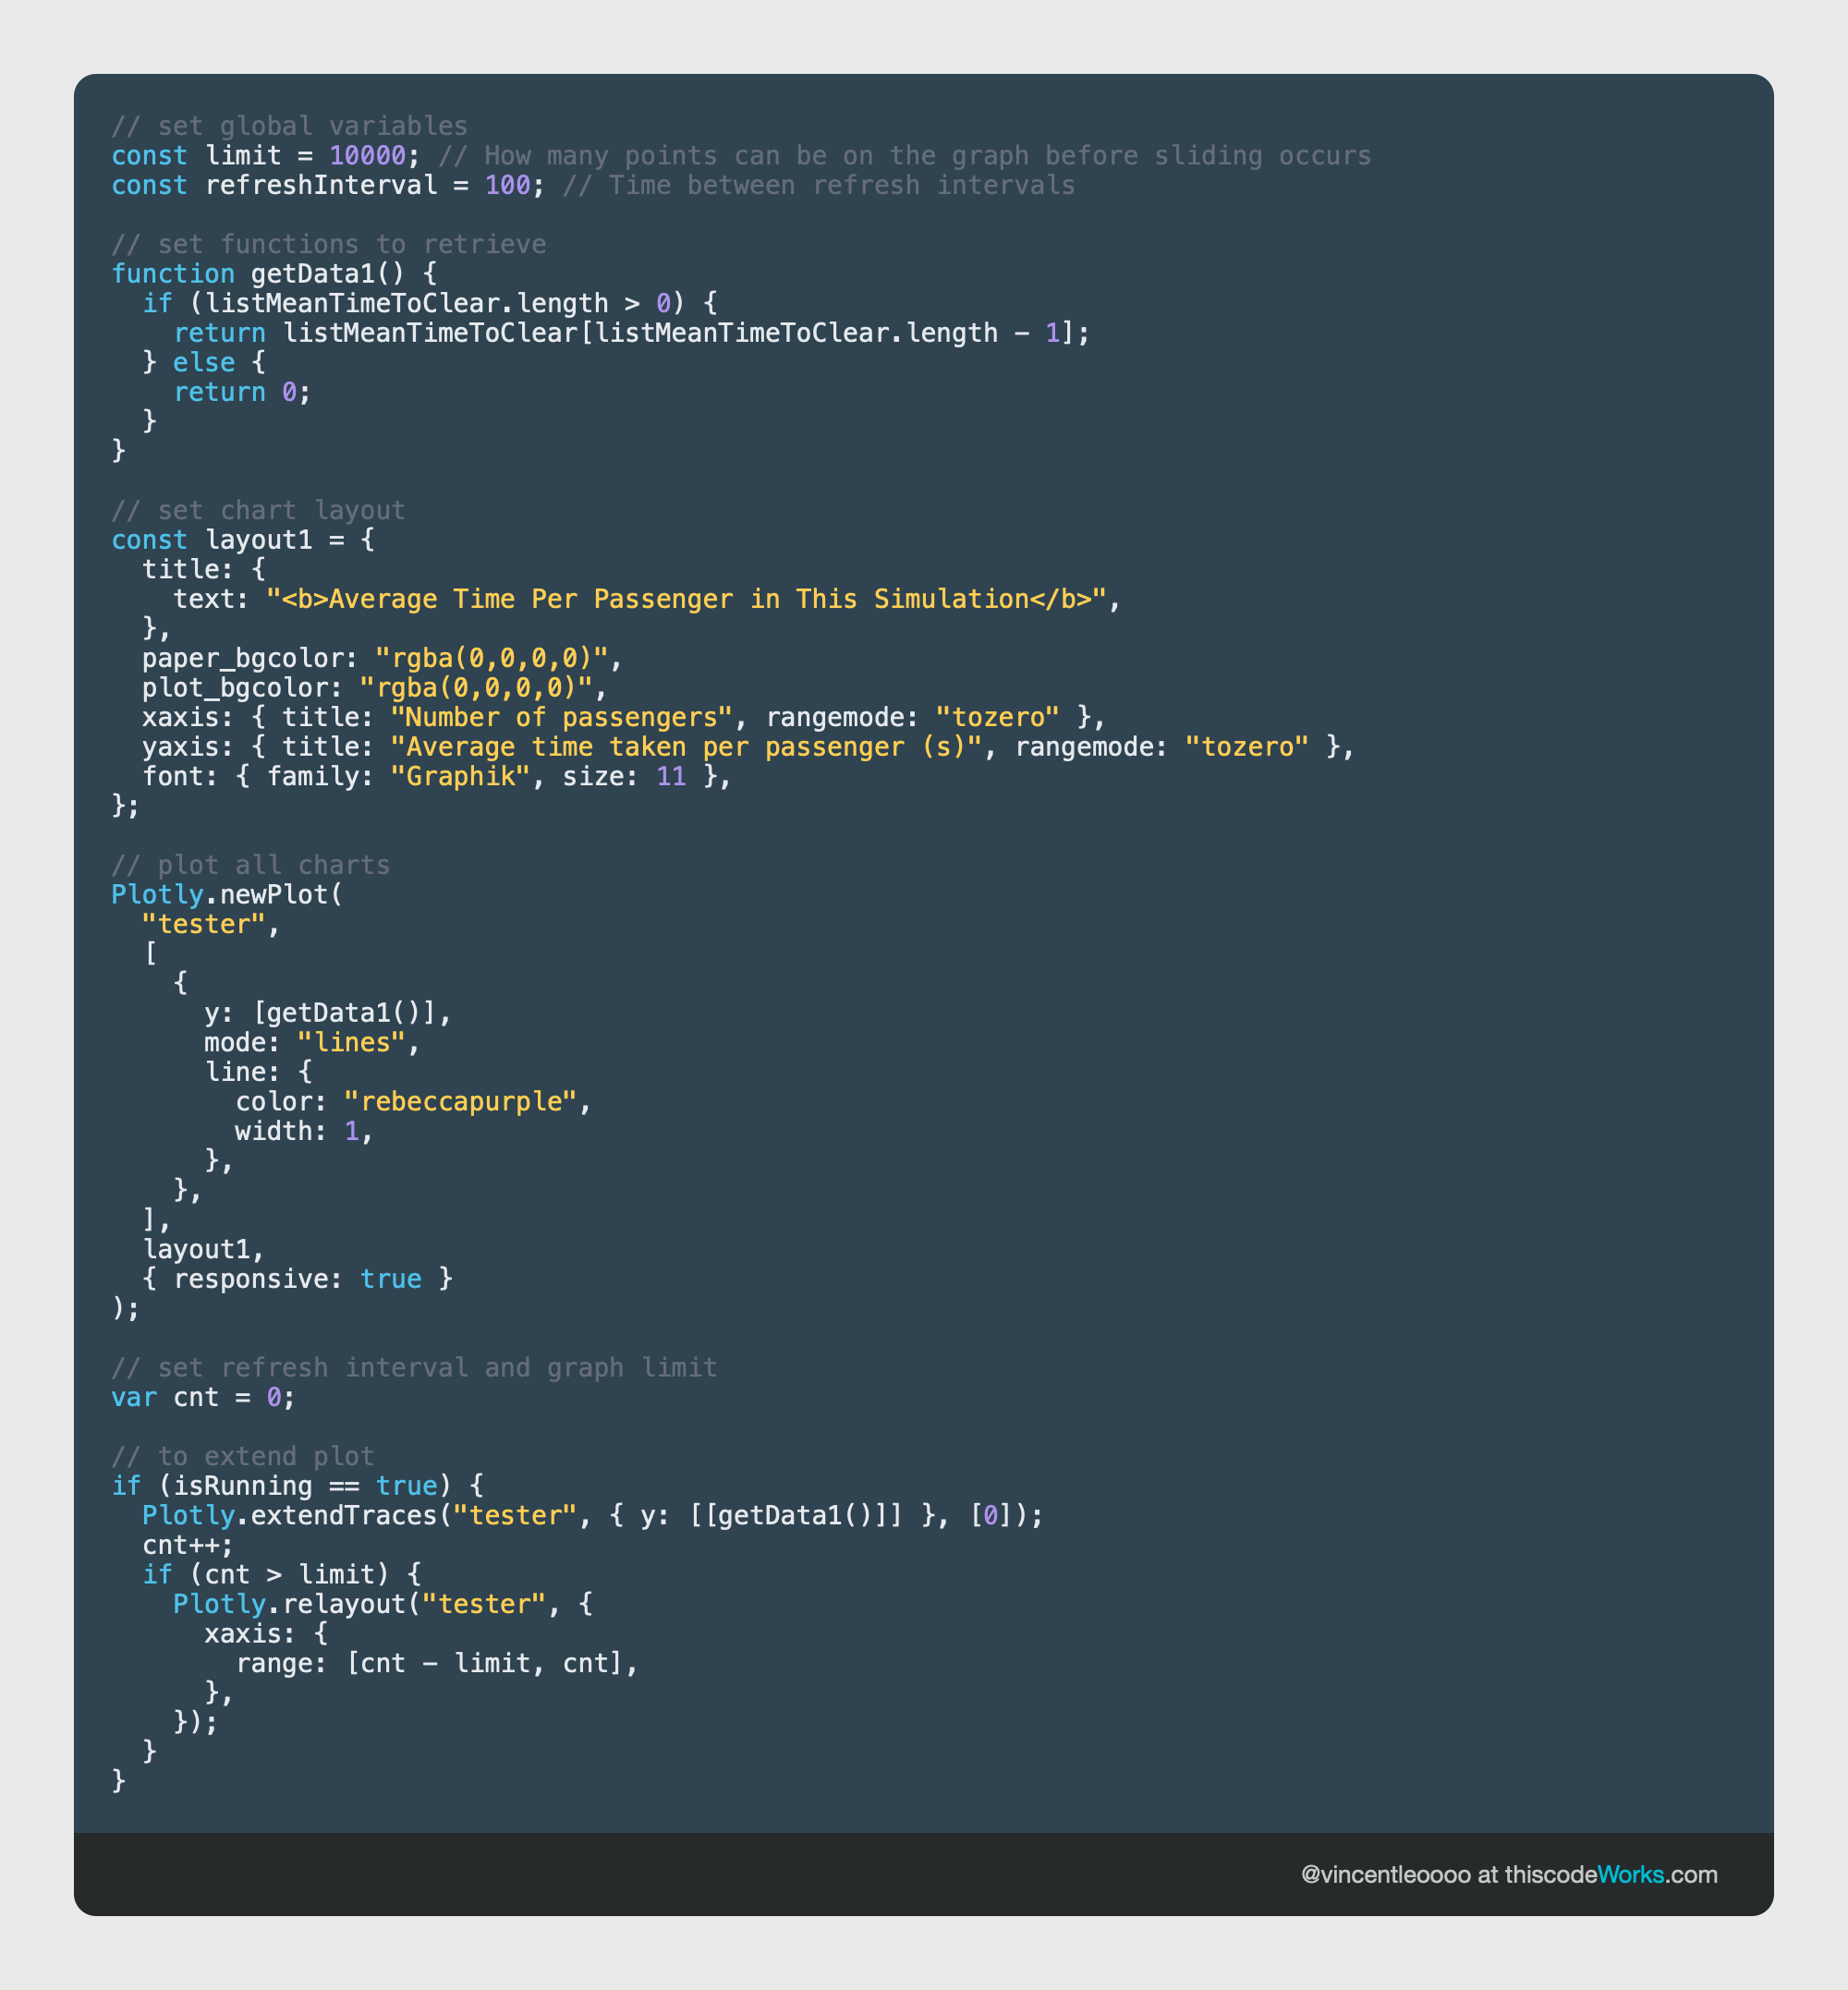
\includegraphics[scale=0.09]{../img/plotly}\caption{Plots code}
	\end{figure}
\end{frame}

\subsubsection*{Downloads}
\begin{frame}{Downloads}
	The downloading function takes in the CSV string and converts it to be downloaded as a proper CSV file.
	\begin{figure}
		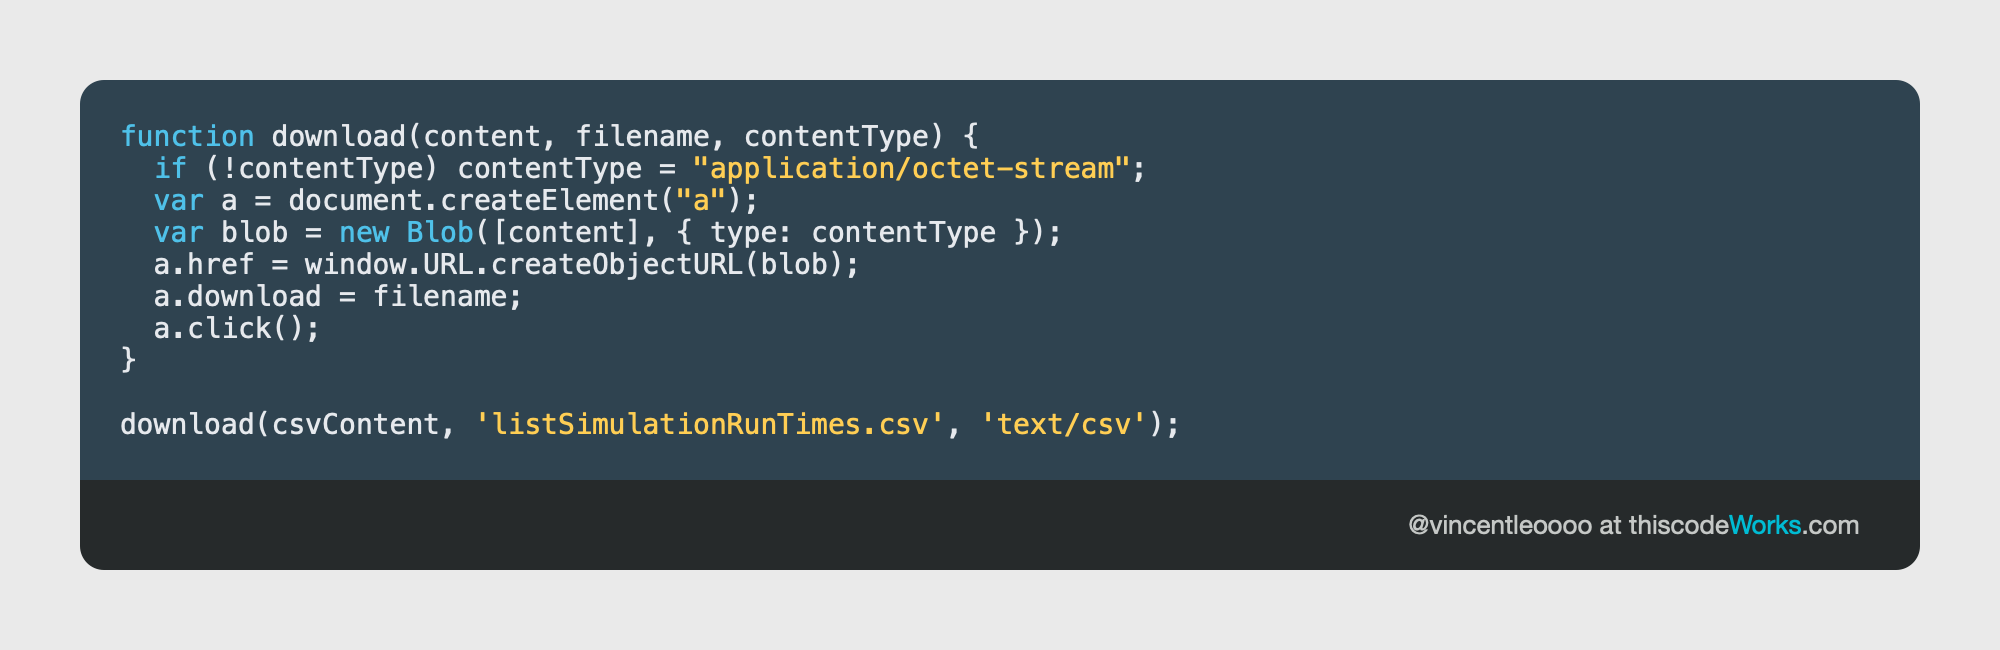
\includegraphics[width=\linewidth]{../img/download-csv}\caption{Downloads code}
	\end{figure}
\end{frame}

\end{document}
